\documentclass[a4paper]{sciposter}
\usepackage{lipsum}
\usepackage{epsfig}
\usepackage{amsmath}
\usepackage{amssymb}
\usepackage{amsthm}
\usepackage[catalan]{babel}
\usepackage{geometry}
\usepackage{multicol}
\usepackage{graphicx}
\usepackage{tikz}
\usepackage{wrapfig}
\usepackage{gensymb}
\usepackage[utf8]{inputenc}
\usepackage{empheq}
\usepackage{letltxmacro}

\graphicspath{{images/}}

\newtheorem{teorema}{Teorema}

\makeatletter
\def\timeframe#1{\def\@timeframe{#1}}
\def\period#1{\def\@period{#1}}
\let\oldr@@t\r@@t
\def\r@@t#1#2{
\setbox0=\hbox{$\oldr@@t#1{#2\,}$}\dimen0=\ht0
\advance\dimen0-0.2\ht0
\setbox2=\hbox{\vrule height\ht0 depth -\dimen0}
{\box0\lower0.4pt\box2}}
\LetLtxMacro{\oldsqrt}{\sqrt}
\renewcommand*{\sqrt}[2][\ ]{\oldsqrt[#1]{#2} }
\makeatother

\geometry{
 landscape,
 a1paper,
 left=5mm,
 right=50mm,
 top=5mm,
 bottom=50mm,
}
\newcommand*\widefbox[1]{\fbox{\hspace{2em}#1\hspace{2em}}}

\newlength\dlf  % Define a new measure, dlf
\newcommand\alignedbox[2]{
% Argument #1 = before & if there were no box (lhs)
% Argument #2 = after & if there were no box (rhs)
&  % Alignment sign of the line
{
\settowidth\dlf{$\displaystyle #1$}
    % The width of \dlf is the width of the lhs, with a displaystyle font
\addtolength\dlf{\fboxsep+\fboxrule}
    % Add to it the distance to the box, and the width of the line of the box
\hspace{-\dlf}
    % Move everything dlf units to the left, so that & #1 #2 is aligned under #1 & #2
\boxed{#1 #2}
    % Put a box around lhs and rhs
}
}

\usepackage{titlesec}
\titleformat{\section}[block]{\LARGE\bfseries\centering}{}{1em}{\color{blue}}
\titleformat{\subsection}[block]{\Large\bfseries\centering}{}{1em}{\color{blue}}
\titleformat{\subsubsection}[block]{\large\bfseries\centering}{}{1em}{\color{blue}}

\usepackage{graphicx,url}

\begin{document}
\fontfamily{phv}\selectfont

\begin{multicols}{3}
\section{Introducció}
Recordatori de conceptes bàsics de probabilitat i estadística.\\
Una \textbf{població} es una variable aleatoria $X$.\\
Una \textbf{mostra aleatòria} de mida $n$ de $X$ és un conjunt de variables aleatòries $X_1,\dots,X_n$ independents i que compleixen el seguent $\forall A\subset\mathbb{R}, i \in 1,\dots,n:P(X_i \in A) = P(X\in A)$\\
Els \textbf{paràmetres} són característiques numèriques poblacionals que solen ser desconegudes, com
\begin{itemize}
	\item La mitjana $\mu = E(X)$
	\item La variància $\sigma^2 = Var(X)$
	\item La desviació estàndard $\sigma = \sqrt{Var(X)}$
\end{itemize}
\subsection{Estadistics}
Donada una mostra aleatòria $X_1,\dots,X_n$ de $X$, un \textbf{estadístic} és una funció d'aquestes variables, i potser de constants conegudes.\\
\textbf{Exemples:}
La mitjana mostral $\overline{x} = \frac{1}{n} \sum\limits_{i=1}^{n} x_i$.\\
La variància mostral (corregida) $S^2 = \frac{1}{n-1} \sum\limits_{i=1}^{n} (x_i - \overline{x})^2$.\\
La variància mostral (no corregida) $S'^2 = \frac{n-1}{n}S^2$.\\
La quasi-variància mostral $\tilde{S}^2 = \frac{1}{n} \sum\limits_{i=1}^{n} (x_i - \mu)^2$ on $\mu$ és la mitjana poblacional de $X$.
\subsection{Estimadors}
Un \textbf{estimador} és un estadístic que es fa servir per estimar un determinat parametre.\\
Notació: Un estadístic que s'usa per estimar el paràmetre $\theta$ es denotat com $\hat{\theta}$. Llavors tenim
\begin{itemize}
	\item $\hat{\mu} = \overline{X}$.
	\item $\hat{\sigma}^2 = S^2$.
\end{itemize}
Distingim entre \textbf{estimadors} (és variable aleatòria) i \textbf{estimació} (valor concret, que es la seva realització, en minúscula).
\subsection{Distrubucions mostrals més usuals}
Donat un estadístic funció de la mostra $X_1,\dots,X_n$ que és una variable aleatòria, la seva distribució és la \textbf{distribució de mostral de l'estadístic}.\\
Propietats de la llei de la mitjana mostral:
\begin{itemize}
	\item $\mu_{\overline{X}} = E(\overline{X}) = \mu$.
	\item $\sigma^2_{\overline{X}} = Var(\overline{X}) = \frac{\sigma^2}{n}$.
\end{itemize}
Si $X \sim N(\mu,\sigma^2)$, aleshores $\overline{X} \sim N(\mu,\frac{\sigma^2}{n})$.\\
Propietats de la llei de la variància mostral (corregida), sense corregir i quasivariància:
\begin{itemize}
	\item $E(\tilde{S}^2) = \sigma^2$.
	\item $E(S^2) = \sigma^2$.
	\item $E(S'^2) = \frac{n-1}{n}\sigma^2$.
\end{itemize}
Si $X \sim N(\mu,\sigma^2)$, aleshores $\frac{n\tilde{S}^2}{\sigma^2} = \frac{1}{\sigma^2} \sim^n_{i=1}(X_1-\mu)^2 \sim \chi^2_n$, on $\chi^2_n$ és la distribució khi-quadrat amb $n$ graus de llibertat. Això es fa servir si $\mu$ és coneguda.\\
\begin{teorema}[Teorema de Fisher]
Si $X_1, \dots, X_n$ és una mostra aleatòria de $X \sim N(\mu,\sigma^2)$, aleshores:
\begin{enumerate}
	\item $\overline{X}$ i $S^2$ són independents.
	\item A més $\frac{(n-1)S^2}{\sigma^2} = \frac{1}{\sigma^2} \sum\limits_{i=1}^{n} (X_i - \overline{X})^2 \sim \chi^2_{n-1}$.
\end{enumerate}
Aixó es fa servir si $\mu$ és desconeguda.
\end{teorema}
\begin{figure}[H]
    \centering
    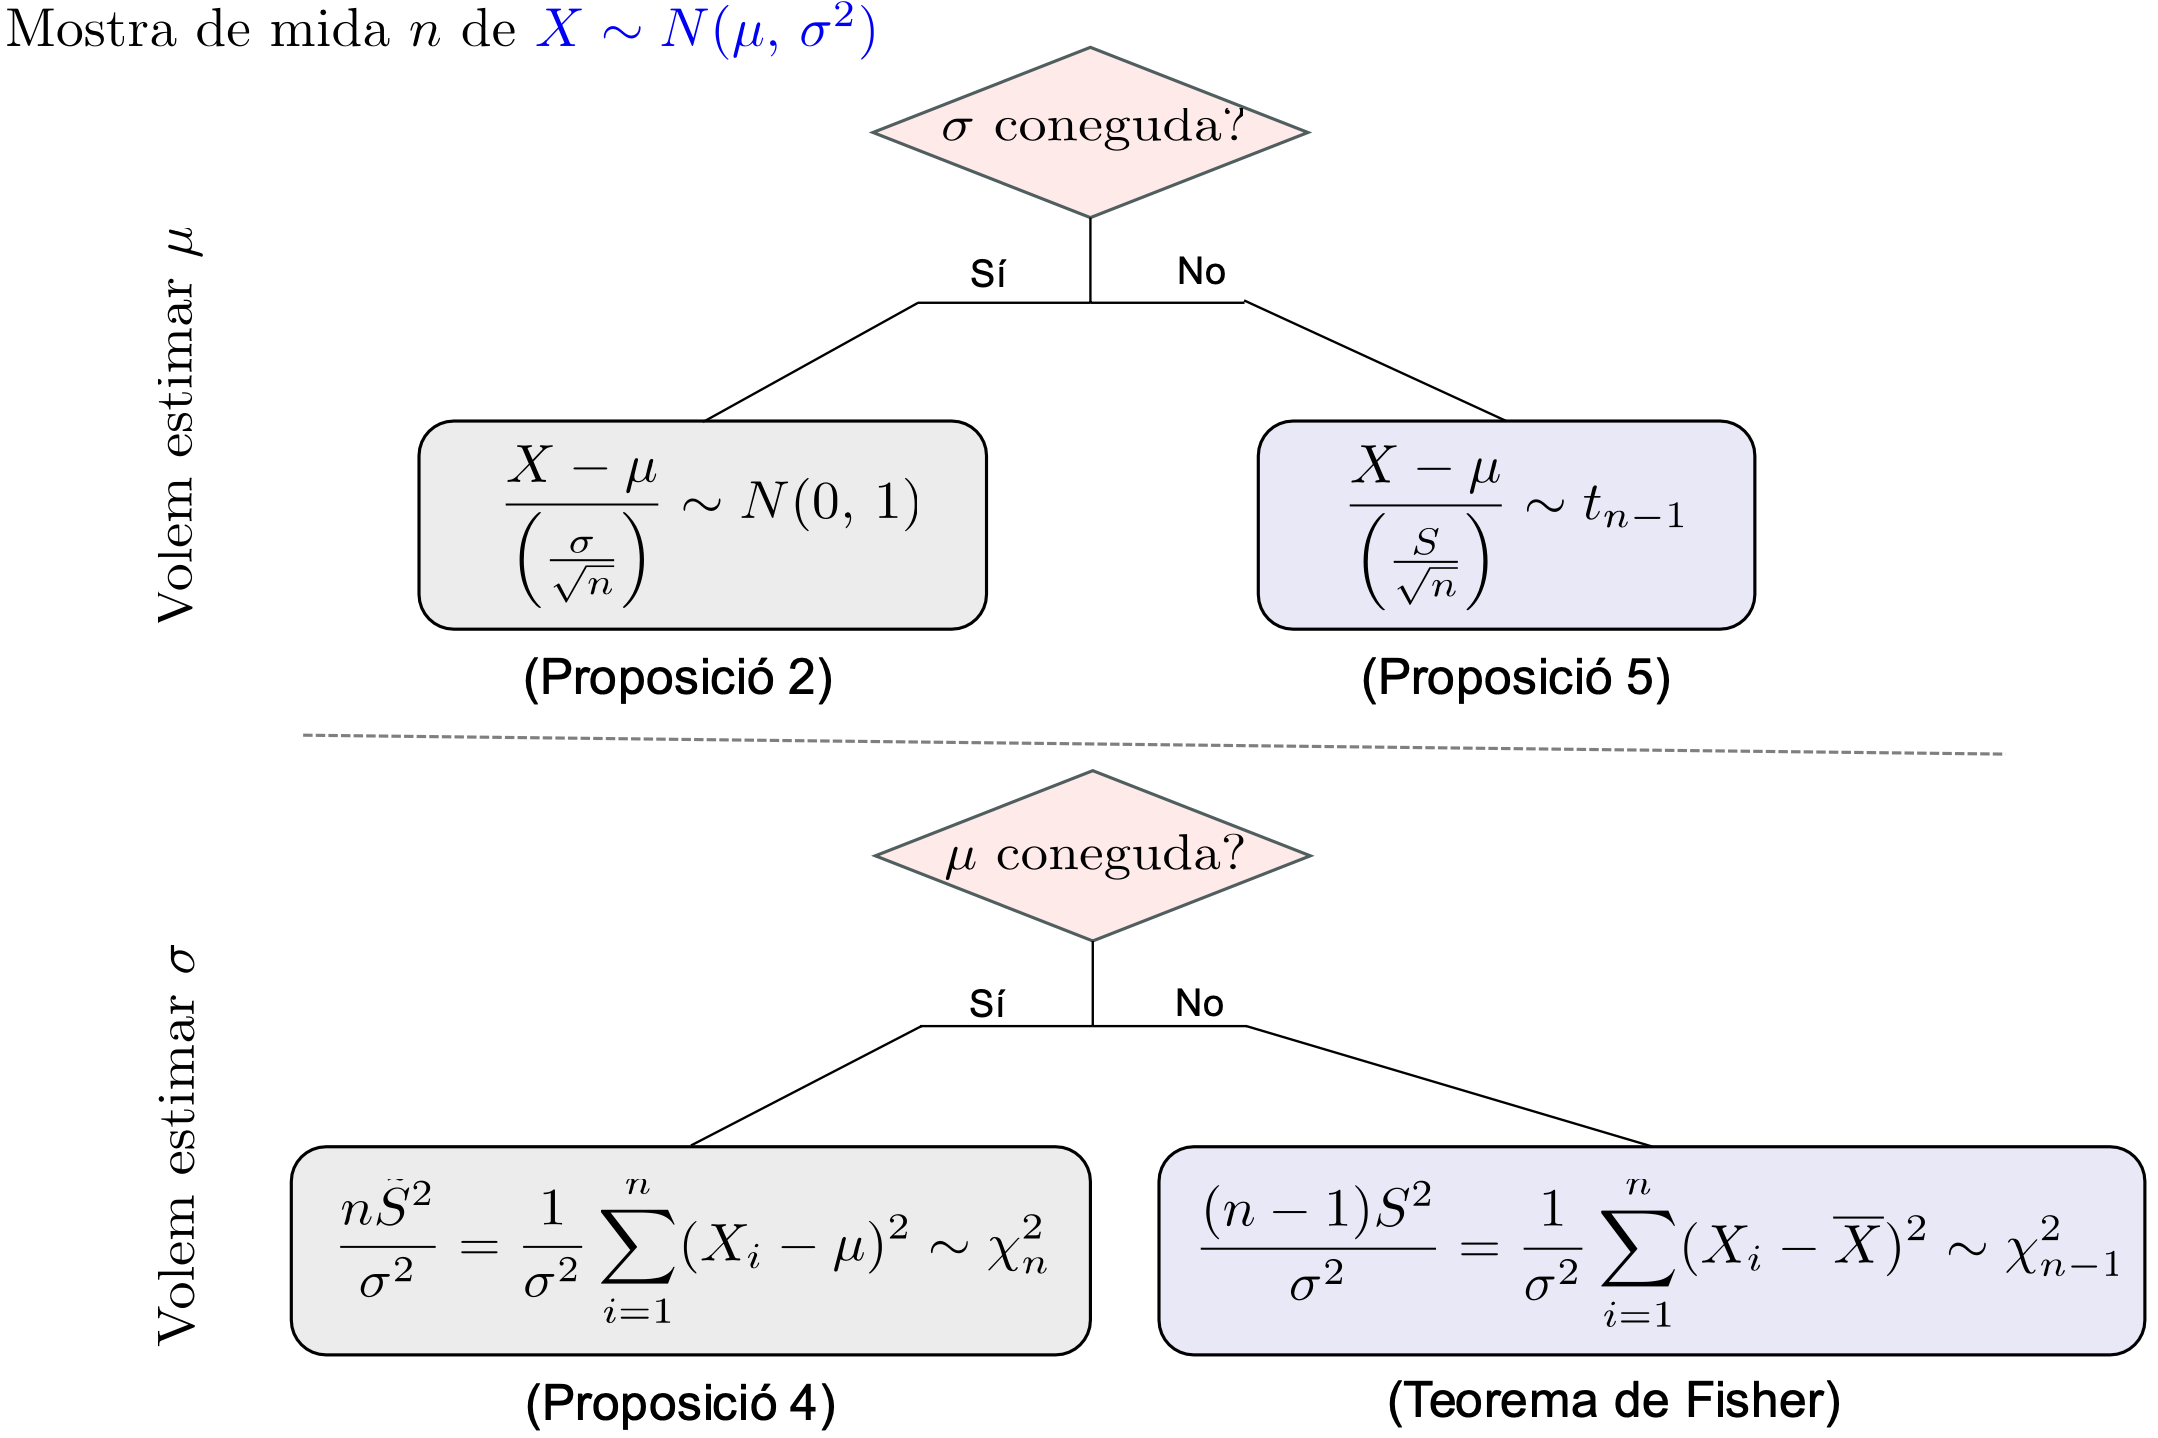
\includegraphics[width=0.8\textwidth]{fix.png}
\end{figure}
Si $X \sim N(\mu, \sigma^2)$ aleshores $T = \frac{\overline{X} - \mu}{\left(\frac{S}{\sqrt{n}}\right)} \sim t_{n-1}$, on $\underbrace{S = +\sqrt{S^2}}_\text{Això es estupid?}$ i $t_{n-1}$ és la distribució t de Student amb $n-1$ graus de llibertat.
\subsection{Distribucions mostrals asimptòtiques}
Si $X_1,\dots,X_n$ és una mostra aleatòria de $X$ amb llei qualsevol i mida $n$ tal que $E(X) = \mu$ i $Var(X) = \sigma^2$, aleshores $\underline{X}_n \approx N\left(\mu, \frac{\sigma^2}{n}\right)$, equivalentment $Z_n = \frac{\overline{X}_n - \mu}{\left(\frac{\sigma}{\sqrt{n}}\right)} \approx N(0,1)$.\\
També si $n$ és prou gran i $\sigma$ és desconeguda, aleshores tenim el seguent $\frac{\overline{X}_n - \mu}{\left(\frac{S_n}{\sqrt{n}}\right)} \approx N(0,1)$. A la majoria de distribucions l'approximació es prou bona a partir de $n \geq 30$.\\
\begin{figure}[H]
	\centering
	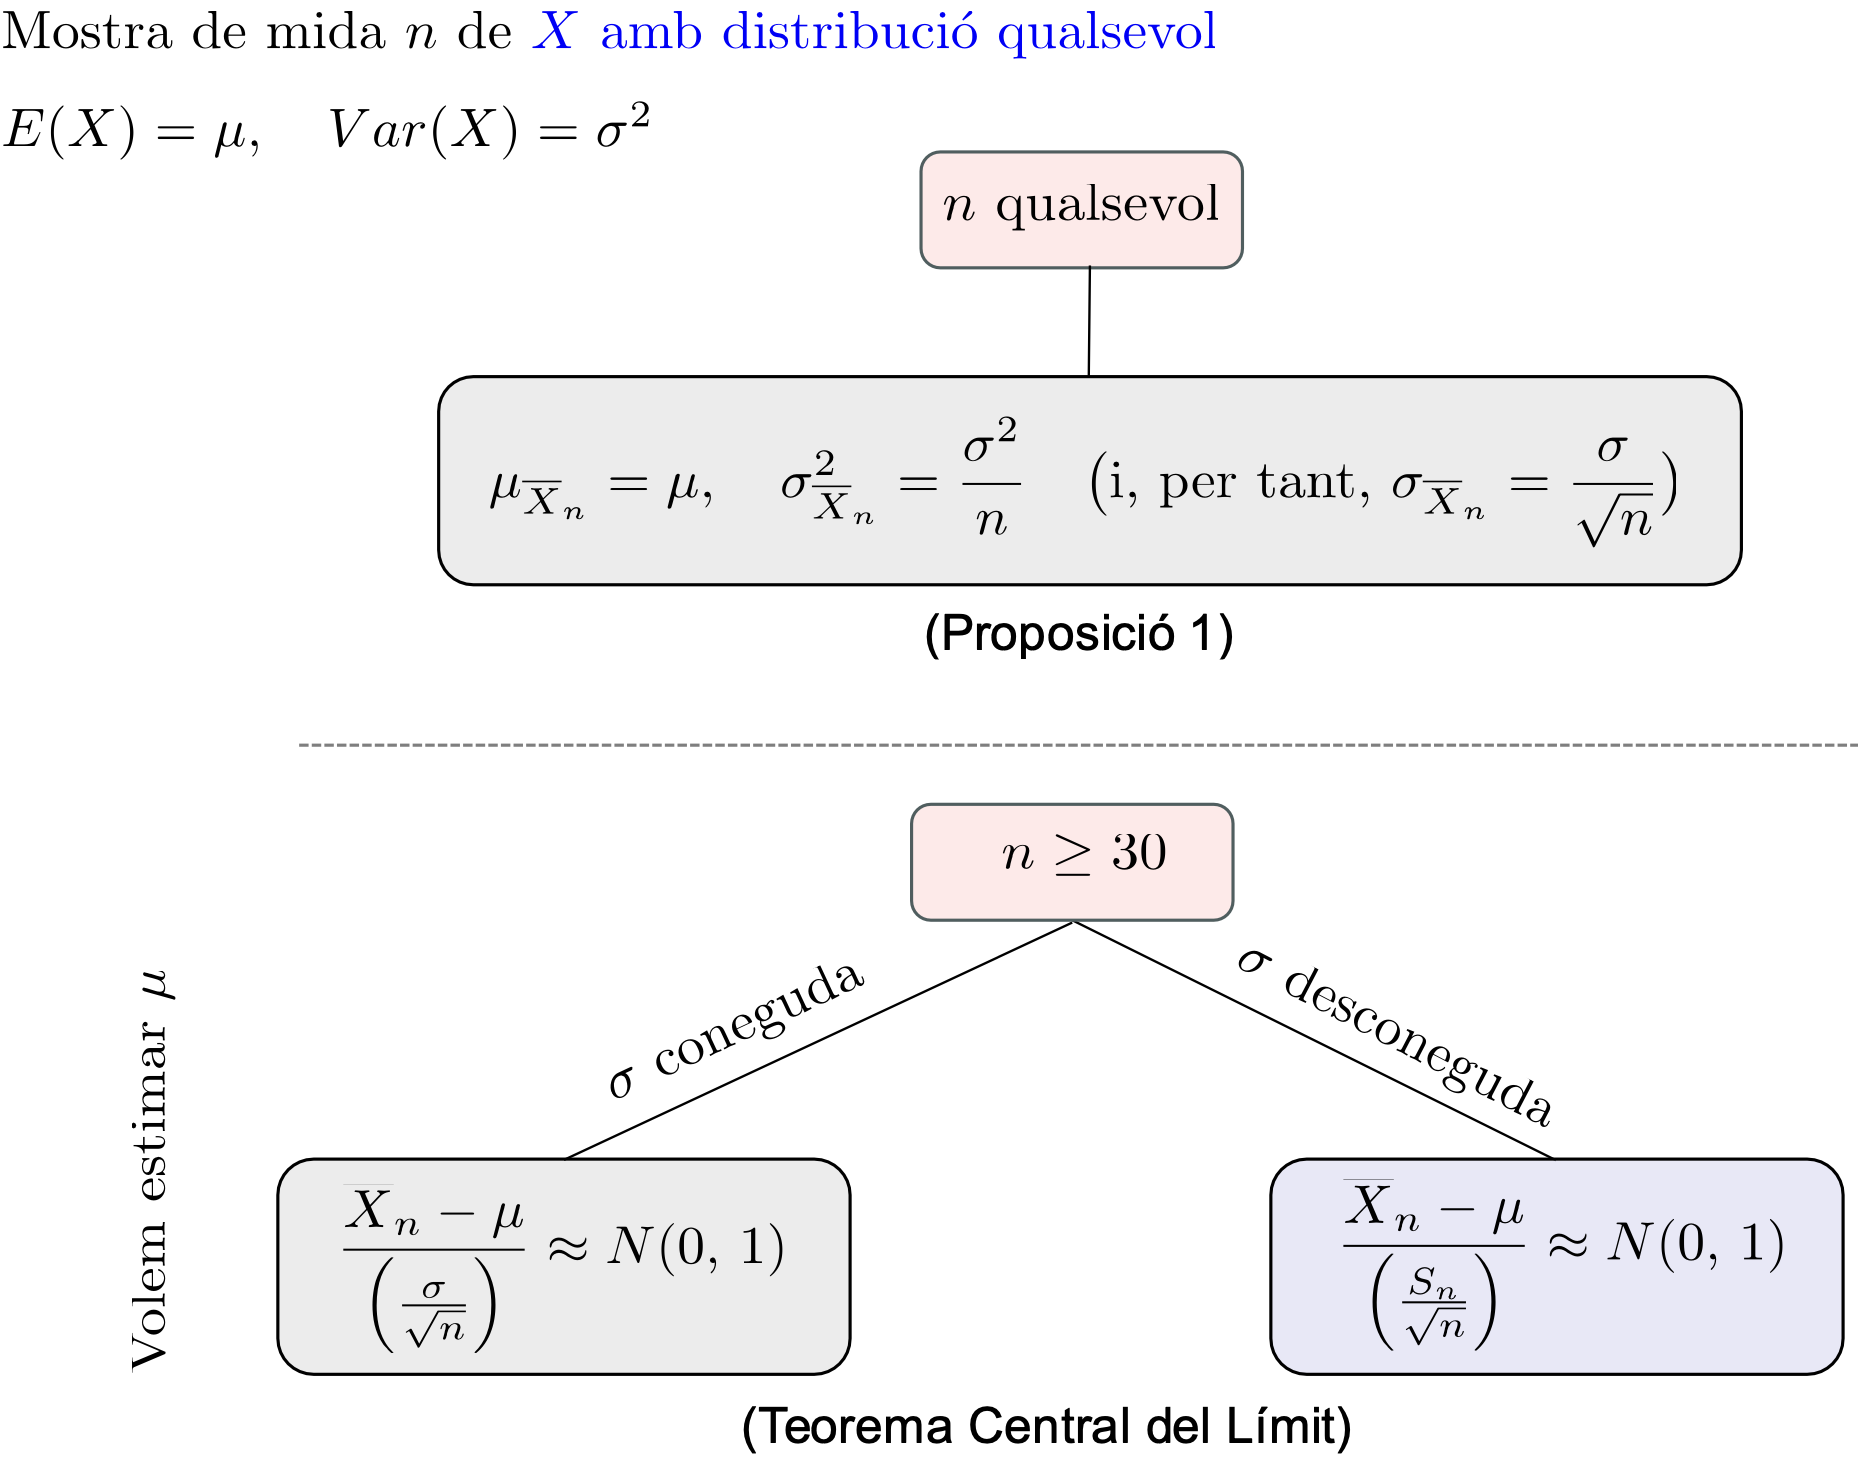
\includegraphics[width=0.8\textwidth]{distro.png}
	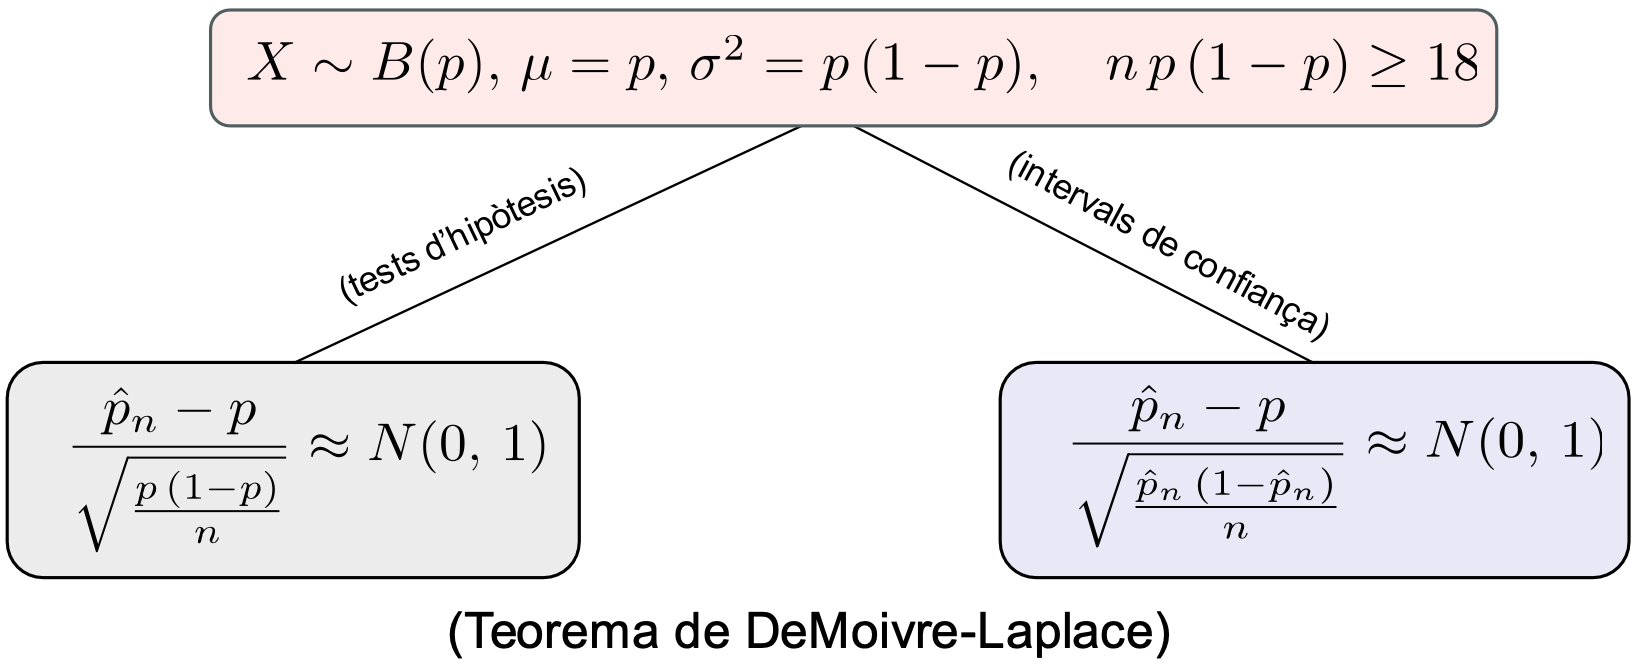
\includegraphics[width=0.8\textwidth]{distro2.png}
\end{figure}
$\frac{\hat{p}_n-p}{\sqrt{\frac{p(1-p)}{n}}} \approx N(0,1)$, on $\hat{p}_n$ és la proporció mostral, $p$ és la proporció poblacional i $n$ és la mida de la mostra.\\
Quan més gran sigui $np(1-p)$ millor es l'aproximació. Es considera acceptable si $np(1-p) \geq 5$.
\subsection{Estadístics d'ordre}
Donada una mostra de mida $n$ de $X$: $X_1,\dots,X_n$, els estadístics d'ordre són les variables aleatòries $X_{(1)},\dots,X_{(n)}$ que són les dades ordenades de menor a major.\\
Exemples importants:
\begin{itemize}
	\item La mediana, el valor que separa la meitat superior de la inferior $Q_2 = \begin{cases}
	X_{((n+1)/2)} & \text{si $n$ és senar} \\
	\frac{X_{(n/2)} + X_{(n/2+1)}}{2} & \text{si $n$ és parell}
	\end{cases}$
	\item Els quartils, els valors que divideixen la mostra en 4 parts iguals: $Q_1 = X_{(n/4)}$, $Q_3 = X_{(3n/4)}$.
	\item El rang interquartílic, $IQR = Q_3 - Q_1$. Ajuda a entendre la dispersió de les dades centrals.
\end{itemize}
Si $X$ és una v.a. amb funció de distribució $F_X$, i $X_1,\dots,X_n$, aleshores la funció de dist. de la v.a. màxim és $F_{X_{(n)}}(t) = (F_X(t))^n\;\forall t \in \mathbb{R}$.\\
Si $X$ és una v.a. amb funció de distribució $F_X$, i $X_1,\dots,X_n$, aleshores la funció de dist. de la v.a. mínim és $F_{X_{(1)}}(t) = 1 - (1 - F_X(t))^n\;\forall t \in \mathbb{R}$.\\
Si $X$ és una v.a. amb funció de distribució $F_X$, i $X_1,\dots,X_n$, aleshores la funció de dist. de la v.a. $k$-èssim és $F_{X_{(k)}}(t) = \sum\limits_{j=k}^{n} \binom{n}{j} (F_X(t))^j (1-F_X(t))^{n-j}\;\forall t \in \mathbb{R}$.
\subsection{Apendix A}
\subsubsection{La distribució $\chi^2$}
Si $Z_1,\dots,Z_n$ són v.a. independents amb distribució $N(0,1)$, aleshores la v.a. $Y = Z_1^2 + \dots + Z_n^2$ llavors $Y \sim \chi^2_n$ amb $n$ graus de llibertat.\\
Propietats:
\begin{itemize}
	\item La variable $Y$ pren valors positius; la seva funció de densitat
	\begin{displaymath}
		f_Y(x) =
		\begin{cases}
			0 & \text{si } x \leq 0 \\
			\frac{1}{2^{n/2}\Gamma(n/2)}x^{n/2-1}e^{-x/2} & \text{si } x > 0
		\end{cases}
	\end{displaymath}
	Amb $\Gamma$ la funció gamma d'Euler.
	\item La seva funció generatriu de moments és $\phi_Y(t) = (1-2t)^{-n/2},\;t<1/2$.
	\item $E(Y) = n$, $Var(Y) = 2n$.
    \item Si $Z \sim N(0,1)$ aleshores $Z^2 \sim \chi^2_1$.
    \item Quan $n$ és suficientment gran es pot fer servir l'aproximació $\sqrt{2\chi^2_n} \approx N(\sqrt{2n-1}, 1)$.
\end{itemize}
\subsubsection{La distribució $t$ de Student}
Si $Z \sim N(0,1)$ i $Y \sim \chi^2_n$ són independents, aleshores la v.a. $T = \frac{Z}{\sqrt{Y/n}}$ $Y \sim t_n$, la $t$ de Student amb $n$ graus de llibertat.\\
Propietats:
\begin{itemize}
	\item La funció de densitat de $T \sim t_n$ és
	\begin{displaymath}
		f_T(x) = \frac{\Gamma\left(\frac{n+1}{2}\right)}{\sqrt{\pi n}\gamma\left(\frac{n}{2}\right)}\left(1+\frac{x^2}{n}\right)^{-\frac{n+1}{2}}
	\end{displaymath}
	\item La densitat de la $t$ de Student és no nul·la en tot $\mathbb{R}$. També és simètrica respecte l'eix vertical. $n \to \infty \Rightarrow t_n \to N(0,1)$.
	\item Si $T \sim t_n$ aleshores $E(T^k)$ només existeix si $k < n$. A més, $E(T) = 0$ si $n > 1$ i $Var(T) = \frac{n}{n-2}$ si $n>2$.
\end{itemize}
\section{Intervals de confiança}
Sigui $X$ una v.a. i $\theta$ qualsevol paràmetre desconegut de la llei de $X$. Fixem un valor $\gamma \in (0,1)$. Un interval de confiança per $\theta$ és una parella de nombres reals $t_1 < t_2$ tals que $\theta$ està entre $t_1$ i $t_2$ amb una confiança de $\gamma$. $\gamma$ és el nivell de confiança de l'interval.\\
Com? Es tracta de trobar dos estadístics $T_1$ i $T_2$ tal que $P(T_1 < \theta < T_2) \geq \gamma$.\\
El metode més comú per trobar intervals de confiança és el mètode del pivot.
\subsection{Mètode del pivot}
Un pivot és una v.a. $T$ tal que és una funció de la mostra i del parametre $\gamma$ i no depén de cap parametre desconegut $T = T(X_1,\dots,X_n;\theta)$. La llei de $T$ és coneguda i no depén de cap paràmetre desconegut excepte $\theta$.
\subsubsection{Per mitjana normal amb variància coneguda}
Tenim una població identificada amb una v.a. $X \sim N(\mu, \sigma^2)$ amb $\sigma > 0$ coneguda però $\mu$ desconeguda. I tenim una mostra de mida $n$ de $X$. Un pivot per a $\mu$ és $Z = \frac{\overline{X} - \mu}{\frac{\sigma}{\sqrt{n}}}$.\\
Llavors, apliquem:
\begin{enumerate}
    \item $P(a\leq Z\leq b) = \gamma$, com $a = -b = z_{\alpha/2}$
    \item Tenim llavors $P(a\leq\frac{\overline{X}-\mu}{\left(\frac{\sigma}{\sqrt{n}}\right)} = \gamma$
    \item Aïllem $\mu$ i obtenim $P(\overline{X} - z_{1-\alpha/2}\frac{\sigma}{\sqrt{n}} \leq \mu \leq \overline{X} + z_{1-\alpha/2}\frac{\sigma}{\sqrt{n}}) = \gamma$ on $\boxed{\alpha = 1-\gamma}$
    \item Finalment, tenim\\$IC_\gamma(\mu) = [t_1, t_2] = [\overline{X} - z_{1-\alpha/2}\frac{\sigma}{\sqrt{n}}, \overline{X} + z_{1-\alpha/2}\frac{\sigma}{\sqrt{n}}]$
\end{enumerate}
S'anomena error de precisió de l'interval de confiança $IC_\gamma(\mu)$ al valor (la constant) $e = z_{1-\alpha/2}\frac{\sigma}{\sqrt{n}}$.
L'error satisfà el seguent
\begin{enumerate}
	\item $P(|\overline{X} - \mu| \leq e) = \gamma$
	\item és la semi-amplitud de l'interval de confiança. Quant més gran és l'error, menys precís l'interval.
	\item Depén de la mida de la mostra $n$, del nivell de confiança $\gamma$ i de la desviació tipica poblacional $\sigma$.
	\begin{enumerate}
		\item L'error és una funció creixent del nivell de confiança.
		\item L'error és una funció creixent de la desviació típica poblacional.
		\item L'error és una funció decreixent de la mida de la mostra.
	\end{enumerate}
	\item Per tal que l'error de precisió d'un interval de confiança sigui el menor menor posible i donat que $\sigma$ és una constant que no podem modificar, ens queden dues opcions:
	\begin{enumerate}
		\item El recurs fonamental és augmentar la mida de la mostra.
		\item L'altre recurs és menys recomenable: disminuir el nivell de confiança.\\
		Però això incrementa el risc de donar un interval que no contingui el paràmetre.
	\end{enumerate}
\end{enumerate}
Si fixem un error màxim $\varepsilon > 0$ i un nivell de confiança, podem trobar la mida de la mostra necessària per aconseguir-ho.\\
Per fer-ho, hem d'aïllar $n$ de la desigualtat $e = z_{1-\alpha/2}\frac{\sigma}{\sqrt{n}} \leq \varepsilon$ i obtenim $n \geq \left(\frac{z_{1-\alpha/2}\sigma}{\varepsilon}\right)^2$.\\
Llavors, agafem el primer nombre enter $n = \left\lceil\left(\frac{z_{1-\alpha/2}\sigma}{\varepsilon}\right)^2\right\rceil$
\subsubsection{Per mitjana normal amb variància desconeguda}
Tenim una població identificada amb una v.a. $X \sim N(\mu, \sigma^2)$ amb $\mu$ i $\sigma > 0$ desconeguda. Llavors tenim un pivot $T = \frac{\overline{X} - \mu}{\frac{S}{\sqrt{n}}}$.\\
on $S = \sqrt{\frac{1}{n-1}\sum\limits_{i=1}^n(X_i - \overline{X})^2}$ és la desviació típica mostral.\\
Si repetim el mateix procediment que abans, obtenim $IC_\gamma(\mu) = [\overline{X} - t_{n-1,1-\alpha/2}\frac{S}{\sqrt{n}}, \overline{X} + t_{n-1,1-\alpha/2}\frac{S}{\sqrt{n}}]$.\\
Notem que l'error serà $e = t_{n-1,1-\alpha/2}\frac{S}{\sqrt{n}}$. Satisfà les mateixes propietats que abans menys que depèn de $S$ en canvi de $\sigma$.\\
Analogament amb abans, si fixem un error màxim $\varepsilon > 0$ i un nivell de confiança, podem trobar la mida de la mostra necessària per aconseguir-ho. Aquesta serà $n = \left\lceil\left(\frac{t_{n-1,1-\alpha/2}S}{\varepsilon}\right)^2\right\rceil$.
\subsubsection{Per variància normal amb mitjana desconeguda}
Suposem que tant $\mu$ com $\sigma^2$ són desconeguts. Llavors, tenim un pivot $\Psi = \frac{(n-1)S^2}{\sigma^2}$.\\
La llei de $\Psi \sim \chi^2_{n-1}$. No podem fer com anteriorment, ja que $\chi^2$ no es simètrica.\\
Llavors tenim $P(a\leq\Psi\leq b) = \gamma$, on $a = \chi^2_{n-1,\alpha/2}$ i $b = \chi^2_{n-1,1-\alpha/2}$.
Aïllem $\sigma^2$ i obtenim $P\left(\frac{(n-1)S^2}{\chi^2_{n-1,1-\alpha/2}} \leq \sigma^2 \leq \frac{(n-1)S^2}{\chi^2_{n-1,\alpha/2}}\right) = \gamma$, es dir $IC_\gamma(\sigma^2) = \left[\frac{(n-1)S^2}{\chi^2_{n-1,1-\alpha/2}}, \frac{(n-1)S^2}{\chi^2_{n-1,\alpha/2}}\right]$\\
I, obviament, $IC_\gamma(\sigma) = \left[\sqrt{\frac{(n-1)S^2}{\chi^2_{n-1,1-\alpha/2}}}, \sqrt{\frac{(n-1)S^2}{\chi^2_{n-1,\alpha/2}}}\right]$
\subsubsection{Per variància normal amb mitjana coneguda}
El pivot es $\Psi = \frac{n\hat{S}^2}{\sigma^2} \sim \chi^2_n$.\\
No es simètrica, fem el mateix que abans i tindrem en aïllar $\sigma^2$ i o $IC_\gamma(\sigma^2) = \left[\frac{n\hat{S}^2}{\chi^2_{n,1-\alpha/2}}, \frac{n\hat{S}^2}{\chi^2_{n,\alpha/2}}\right]$ i $IC_\gamma(\sigma) = \left[\sqrt{\frac{n\hat{S}^2}{\chi^2_{n,1-\alpha/2}}}, \sqrt{\frac{n\hat{S}^2}{\chi^2_{n,\alpha/2}}}\right]$
\subsubsection{Asimptòtics, per mitjana i la proporció, mostres grans}
Si $n$ és prou gran ($n>30$), podem aproximar amb una normal.\\
$\frac{\overline{X}-\mu}{\sigma/\sqrt{n}} \approx \frac{\overline{X}-\mu}{S/\sqrt{n}} \sim N(0,1)$ ja que $S$ és un estimador de $\sigma$.\\
Si fem servir com pivot $IC_\gamma(\mu) = \left[\overline{X} - z_{1-\alpha/2}\frac{S}{\sqrt{n}}, \overline{X} + z_{1-\alpha/2}\frac{S}{\sqrt{n}}\right]$ i $IC_\gamma(\mu) = \left[\overline{X} - z_{1-\alpha/2}\frac{S}{\sqrt{n}}, \overline{X} + z_{1-\alpha/2}\frac{S}{\sqrt{n}}\right]$ respectivament.\\
Si tenim una població dicotomica $X \sim B(p)$ i ens interesa trobar $p$ tenim el seguent pivot $\frac{\hat{p}-p}{\sqrt{\frac{\hat{p}(1-\hat{p})}{n}}} \approx N(0,1)$, on $\hat{p} = \overline{X}$. Llavors tenim el seguent interval de confiança $IC_\gamma(p) = \left[\hat{\hat{p}}-z_{1-\alpha/2}\sqrt{\frac{\hat{\hat{p}}(1-\hat{\hat{p}})}{n}}, \hat{\hat{p}}+z_{1-\alpha/2}\sqrt{\frac{\hat{\hat{p}}(1-\hat{\hat{p}})}{n}}\right]$ on $\hat{\hat{p}} = \overline{x}$ és la realització de $\hat{p} = \overline{X}$. S'aplica si $n\hat{\hat{p}}(1-\hat{\hat{p}}) \geq 18$\\
Això s'interpreta de forma analoga a abans. L'error de precisió serà $e = z_{1-\alpha/2}\sqrt{\frac{\hat{\hat{p}}(1-\hat{\hat{p}})}{n}}$ i si volem determinar la mida de la mostra tenim $n = \left\lceil\left(\frac{z_{1-\alpha/2}}{2\varepsilon}\right)^2\right\rceil$.
\subsection{IC per la desigualtat de Txebixov}
Sigui $X_1, \ldots, X_n$ una mostra de $X$. Volem estimar $\mu$ però no es prou gran per aproximar-ho via normal.\\
Llavors tenim $IC_\gamma(\mu) = \left[\overline{X} - \sqrt{\frac{\widehat{Var(X)}}{n\alpha}}, \overline{X} + \sqrt{\frac{\widehat{Var(X)}}{n\alpha}}\right]$ on $\widehat{Var(X)}$ és una bona aproximació de $\sigma^2$. Sí fos coneguda podem fer servir $\sigma^2$ en canvi de $\widehat{Var(X)}$.
\subsection{IC per comparar dues poblacions}
Dos poblacions: $X^{(1)}$ i $X^{(2)}$ amb mitjanes $\mu_1$ i $\mu_2$, variàncies $\sigma_1^2$ i $\sigma_2^2$ respectivament.\\
\subsubsection{amb mostres independents}
La variança es coneguda:\\
Considerem $X^{(1)} \sim N(\mu_1, \sigma^2_1)$ i $X^{(2)} \sim N(\mu_2, \sigma^2_2)$.\\
Aleshores tenim que $E(\overline{X}^{(1)} - \overline{X}^{(2)}) = \mu_1 - \mu_2$ i $Var(\overline{X}^{(1)} - \overline{X}^{(2)}) = \frac{\sigma^2_1}{n_1} + \frac{\sigma^2_2}{n_2}$.\\
i a més tenim $\overline{X}^{(1)} - \overline{X}^{(2)} \sim N(\mu_1 - \mu_2, \sigma^2_1/n_1 + \sigma^2_2/n_2)$\\
Podem agafar la seguent funció pivot: $Z = \frac{(\overline{X}^{(1)} - \overline{X}^{(2)}) - (\mu_1 - \mu_2)}{\sqrt{\frac{\sigma^2_1}{n_1} + \frac{\sigma^2_2}{n_2}}} \sim N(0,1)$\\
Fem com sempre i tenim el seguent $IC_\gamma(\mu_1 - \mu_2) =$\\$\left[(\overline{x}_1 - \overline{X}_2) - z_{1-\alpha/2}\sqrt{\frac{\sigma^2_1}{n_1} +\frac{\sigma^2_2}{n_2}},(\overline{x}_1 - \overline{X}_2) + z_{1-\alpha/2}\sqrt{\frac{\sigma^2_1}{n_1} + \frac{\sigma^2_2}{n_2}}\right]$\\
Important: Si les variables no son normals pero $n_1, n_2 > 30$ podem fer servir aquesta aproximació.\\
La variança no es coneguda pero que es poden suposar iguals:\\
Si suposem que $\sigma^2_1 = \sigma^2_2 = \sigma^2$ tenim que $\overline{X}^{(1)} - \overline{X}^{(2)} \sim N(\mu_1 - \mu_2, \sigma^2(1/n_1 + 1/n_2))$\\
Llavors estimem $\sigma^2$ amb $S^2 = \frac{(n_1-1)S_1^2 + (n_2-1)S_2^2}{n_1 + n_2 - 2}$ i tenim que $T = \frac{(\overline{X}_1 - \overline{X}_2) - (\mu_1 - \mu_2)}{S\sqrt{1/n_1 + 1/n_2}} \sim t_{n_1 + n_2 - 2}$\\
Llavors tenim $IC_\gamma(\mu_1 - \mu_2) =$\\$\left[\begin{aligned}[t](\overline{x}_1 - \overline{x}_2) &- t_{n_1 + n_2 - 2, 1-\alpha/2}S\sqrt{1/n_1 + 1/n_2},\\ &(\overline{x}_1 - \overline{x}_2) + t_{n_1 + n_2 - 2, 1-\alpha/2}S\sqrt{1/n_1 + 1/n_2}\end{aligned}\right]$\\
Important: Si $n_1, n_2 > 30$ podem canviar $t_{n_1 + n_2 - 2, 1-\alpha/2}$ per $z_{1-\alpha/2}$.\\
Per variancies desconegudes que NO es poden suposar iguals:\\
Llavors tenim que $T = \frac{(\overline{X}_1 - \overline{X}_2) - (\mu_1 - \mu_2)}{\sqrt{\frac{S_1^2}{n_1} + \frac{S_2^2}{n_2}}}$ que té distribució \textbf{aproximadament} $t_\nu$ on $\nu = \left\lceil\frac{\left(\frac{S^2_1}{n_1}+\frac{S_2^2}{n_2}\right)^2}{\frac{\left(\frac{S^2_1}{n_1}\right)^2}{n_1-1}+\frac{\left(\frac{S^2_2}{n_2}\right)^2}{n_2-1}}\right\rceil$ %me voy a suicidar
Llavors, com sempre, fem $IC_\gamma(\mu_1 - \mu_2) =$\\$\left[(\overline{x}_1 - \overline{x}_2) - t_{\nu, 1-\alpha/2}\sqrt{\frac{S_1^2}{n_1} + \frac{S_2^2}{n_2}},(\overline{x}_1 - \overline{x}_2) + t_{\nu, 1-\alpha/2}\sqrt{\frac{S_1^2}{n_1} + \frac{S_2^2}{n_2}}\right]$\\
I com abans, si $n_1, n_2 > 30$ podem canviar $t_{\nu, 1-\alpha/2}$ per $z_{1-\alpha/2}$.
Per al quocient de variàncies amb poblacions normals. Com les dues son normals, sabem que $U_1 = \frac{(n_1-1)S_1^2}{\sigma^2_1} \sim \chi^2_{n_1-1}$ i $U_2 = \frac{(n_2-1)S_2^2}{\sigma^2_2} \sim \chi^2_{n_2-1}$. Fem servir la distro $F$ de Fisher-Hipercor, llavors tenim $F = \frac{S_1^2/\sigma^2_1}{S_2^2/\sigma^2_2} \sim F_{n_1-1,n_2-1}$. La fem pivotar i llavors $IC_\gamma(\frac{\sigma_2^2}{\sigma_1^2}) = \left[\frac{S_2^2}{S_1^2}F_{n_1-1,n_2-1,\alpha/2},\frac{S_2^2}{S_1^2}F_{n_1-1,n_2-1,1-\alpha/2}\right]$\\
Aquest interval no es simètric. No es gens robust en front a la manca de normalitat.\\
Asimptòtic per a la diferencia de proporcions amb poblacions binàries:
Suposem que $X^{(1)} \sim B(p_1)$ i $X^{(2)} \sim B(p_2)$, son independents. Denotem $\overline{X}_1 = \hat{p}_1$ i $\overline{X}_2 = \hat{p}_2$. Llavors tenim que la seguent funció pivot $\frac{\hat{p}_1 - \hat{p}_2 - (p_1 - p_2)}{\sqrt{\overline{p}(1-\overline{p})(1/n_1 + 1/n_2)}} \sim N(0,1)$ on $\overline{p} = \frac{n_1\hat{p}_1 + n_2\hat{p}_2}{n_1 + n_2}$. Es necesita que $n_1\hat{\hat{p}}_1(1-\hat{\hat{p}}_1) \geq 18$ i $n_2\hat{\hat{p}}_2(1-\hat{\hat{p}}_2) \geq 18$.
Llavors tenim $IC_\gamma(p_1 - p_2) = (\hat{\hat{p}}_1 - \hat{\hat{p}}_2) \pm z_{1-\alpha/2}\sqrt{\overline{\overline{p}}(1-\overline{\overline{p}})(1/n_1 + 1/n_2)}$, sent $\overline{\overline{p}} = \frac{n_1\hat{\hat{p}}_1 + n_2\hat{\hat{p}}_2}{n_1 + n_2}$.
\subsubsection{Dades aparellades}
Si $X_1^{(1)},\dots,X_n^{(1)}$ i $X_1^{(2)},\dots,X_n^{(2)}$ son mostres aleatòries de mida $n$ sent $X^{(1)} \sim N(\mu_1,\sigma_1^2)$ i $X^{(2)} \sim N(\mu_2,\sigma_2^2)$, es diuen aparellades si hi ha dependencia $\forall i = 1,\dots,n$.\\
Llavors, es calculen diferencies $D_1 = X_1^{(1)} - X_1^{(2)},\dots,D_n = X_n^{(1)} - X_n^{(2)}$, amb $D \sim N(\mu = \mu_1-\mu_2, \sigma^2)$ on $\sigma^2$ es desconeguda, ja que no savem la covariancia.\\
Llavors tenim $IC_\gamma(\mu_1 - \mu_2) = \overline{d} \pm t_{n-1,1-\alpha/2}\frac{S_D}{\sqrt{n}}$ on $\overline{d}$ i $S_D$ son mitjana i desviació mostral respectivament.
\subsection{Apendix B}
\subsubsection{Distribució $F$ de Fisher-Hipercor}
Si $X \sim \chi^2_n$ i $Y \sim \chi^2_m$ son independents, llavors la variable aleatòria $F = \frac{X/n}{Y/m}$ es diu que te distribució $F$ de Fisher-Hipercor amb $n$ i $m$ graus de llibertat.
Propietats:
\begin{itemize}
	\item La funció de densitat es\\ $f_F(x) = \frac{\Gamma(\frac{n+m}{2})}{\Gamma(\frac{n}{2})\Gamma(\frac{m}{2})}(\frac{n}{m})^{n/2}x^{n/2-1}\left(1+\frac{n}{m}x\right)^{-(n+m)/2}$ quan $x\geq 0$
	\item $P(F_{n,m}\leq x) = P(F_{m,n}\leq \frac{1}{x}$, aixó serveix per exemple quan $P(F \leq x) = 0.05 \Rightarrow P(F \geq x) = 0.95 =  P(F \leq \frac{1}{x})$
\end{itemize}
\end{multicols}
\end{document}
